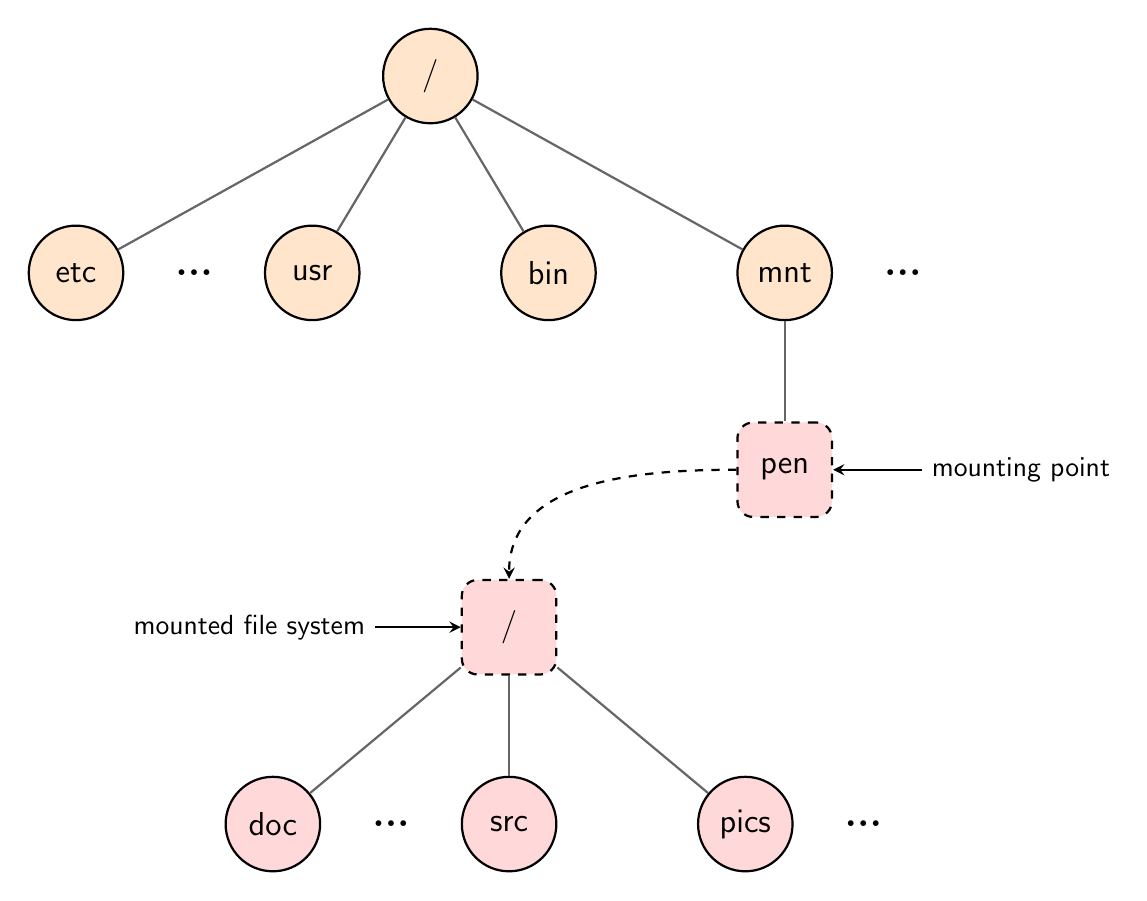
\begin{tikzpicture}[
    % Estilos de los nodos (colores suaves como en tu imagen)
    mainfs/.style={circle, draw=black, thick, fill=orange!20, minimum size=1.2cm, font=\sffamily\large},
    mountfs/.style={circle, draw=black, thick, fill=red!15, minimum size=1.2cm, font=\sffamily\large},
    mountbox/.style={rectangle, rounded corners=2mm, draw=black, thick, dashed, fill=red!15, minimum size=1.2cm, font=\sffamily\large},
    texto/.style={font=\sffamily, text=black},
    line/.style={-, thick, draw=gray!80!black},
    arrow/.style={->, thick, >=stealth, draw=black}
]

% --- SISTEMA DE FICHEROS PRINCIPAL ---
\node[mainfs] (root1) at (0, 0) {/};

\node[mainfs] (etc) at (-4.5, -2.5) {etc};
\node[font=\bfseries\Large] at (-3, -2.5) {...};
\node[mainfs] (usr) at (-1.5, -2.5) {usr};
\node[mainfs] (bin) at (1.5, -2.5) {bin};
\node[mainfs] (mnt) at (4.5, -2.5) {mnt};
\node[font=\bfseries\Large] at (6, -2.5) {...};

\draw[line] (root1) -- (etc);
\draw[line] (root1) -- (usr);
\draw[line] (root1) -- (bin);
\draw[line] (root1) -- (mnt);

% --- PUNTO DE MONTAJE (pen) ---
\node[mountbox] (pen) at (4.5, -5) {pen};
\draw[line] (mnt) -- (pen);

\node[texto] (pentext) at (7.5, -5) {mounting point};
\draw[arrow] (pentext.west) -- (pen.east);

% --- SISTEMA DE FICHEROS MONTADO ---
\node[mountbox] (root2) at (1, -7) {/};

\node[texto] (root2text) at (-2.3, -7) {mounted file system};
\draw[arrow] (root2text.east) -- (root2.west);

% Flecha curva punteada de 'pen' al nuevo '/'
\draw[->, thick, dashed, >=stealth, draw=black] (pen.west) to[out=180, in=90] (root2.north);

% --- HIJOS DEL SISTEMA MONTADO ---
\node[mountfs] (doc) at (-2, -9.5) {doc};
\node[font=\bfseries\Large] at (-0.5, -9.5) {...};
\node[mountfs] (src) at (1, -9.5) {src};
\node[mountfs] (pics) at (4, -9.5) {pics};
\node[font=\bfseries\Large] at (5.5, -9.5) {...};

\draw[line] (root2) -- (doc);
\draw[line] (root2) -- (src);
\draw[line] (root2) -- (pics);

\end{tikzpicture}